\begin{frame}{Primene - Programiranje vodjeno primerima}
    \begin{figure}
        \begin{center}
            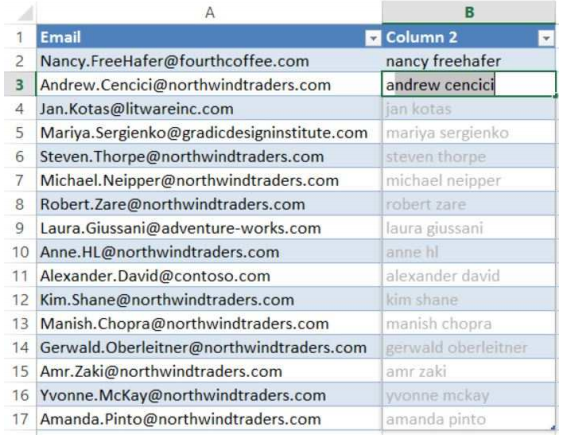
\includegraphics[scale=0.5]{../resources/PBE.PNG}
        \end{center}
        \caption{Automatske transformacije alata FlashFill sprovedene na osnovu par primera zadatih od strane korisnika}
    \end{figure}
\end{frame}

\begin{frame}{Neke od oblasti primene sinteze programa}
    \begin{itemize}
        \item Priprema podataka
        \item Grafika
        \item Sugestije prilikom kodiranja
        \item Superoptimizacija
        \item Konkurentno programiranje
        \item Popravka koda
    \end{itemize}
\end{frame}

\begin{frame}[fragile]{Primene - Popravka koda - Primer}
    \begin{figure}[!h]
        \centering
        \tiny
        \begin{tabular}{ccc|cc}
            \multicolumn{3}{c|}{Ulaz} & \multicolumn{2}{c}{Izlaz}\\
            inb & usep & dsep & expected & actual \\
            \hline
            1 & 0 & 100 & 0 & 0 \\
            1 & 11 & 110 & 1 & 0 \\
            0 & 100 & 50 & 1 & 1 \\
            1 & -20 & 60 & 1 & 0 \\
            0 & 0 & 10 & 0 & 0 \\
        \end{tabular}

        \centering
        \begin{lstlisting}[language=C, basicstyle=\tiny]
            int buggy(int inb, int usep, int dsep)
            {
                int bias;
                if (inb)
                    bias = dsep; //fix: bias = usep+100
                else
                    bias = usep;
                if (bias > dsep)
                    return 1;
                else
                    return 0;
            }
        \end{lstlisting}

        \caption{Primer koda sinteziranog od strane programa \emph{SemFix} koristeći skup ulaznih i izlaznih test primera.}
        \label{fig:CodeRepair}
    \end{figure}
\end{frame}





\iffalse
\begin{frame}{Primene - Popravka koda}
    \begin{itemize}
        \item Računanje modifikacija programa $P$ koje stvaraju nov program $P'$ takav da zadovoljava specifikaciju $\phi$
        \item Ubacuju se alternativni izbori za izraze u programu
        \item Tehnikama programske sinteze izraza pronađu izrazi koji program dovode u oblik koji zadovoljava $\phi$
    \end{itemize}
\end{frame}

\begin{frame}{Primene - Sugestije prilikom kodiranja}
    \begin{itemize}
        \item Podrške okruženja za rad:
        \begin{itemize}
            \item \emph{IntelliSense} za \emph{MS Visual Studio}
            \item \emph{Content Assist} za \emph{Eclipse}
        \end{itemize}
        \item Tehnike za generisanje čitavih jedinica koda:
        \begin{itemize}
            \item \emph{statistički modeli}
            \item \emph{dopuna usmerena tipovima} (eng. \emph{type-directed completion})
            \item ostale tehnike (koriste ih \emph{InSynth} i \emph{Bing Developer Assistant})
        \end{itemize}
    \end{itemize}
\end{frame}

\begin{frame}{Primene - Grafika}
    \begin{itemize}
        \item Konstrukcija ponovljenih objekata
        \item Korišćenjem PBE, korisnik prikaže par primera a sintezer predviđa naredne objekte u nizu
        \item Interaktivno postavljanje grafičkih objekata preko grafičkog interfejsa
        \item Efikasnija geometrijska izračunavanja, brže animacije
    \end{itemize}
\end{frame}

\begin{frame}{Primene - Superoptimizacija}
    \begin{itemize}
        \item Kreiranje optimalnog poretka instrukcija mašinskog koda zarad dobijanja na performansama
        \item Primer
        \begin{figure}[!h]
            \centering
            \small
            \begin{tabular}{rl}
                originalni kod: & $\mathit{prosek}=\frac{x+y}{2}$\\
                optimizovani kod: & prosek = $(x \mid y)-((x \oplus y) \gg 1)$
            \end{tabular}
        \end{figure}
        \item Jedan od načina da se kod automatski optimizuje je korišćenje  \emph{enumerativne pretrage}
    \end{itemize}
\end{frame}

\begin{frame}{Primene - Konkurentno programiranje}
    \begin{itemize}
        \item Pomoć pri pisanju bezbednog kompleksnog višenitnog koda
        \item \emph{Sinteza vođena apstrakcijom}:
        \begin{itemize}
            \item Pravi se apstraktna reprezentacija programa u apstraktnom domenu
            \item Proverava se da li postoji kršenje postavljene specifikacije programa (obično trka za podacima)
            \item Ukoliko postoji prekršenje, menjamo ili apstrakciju (npr. sužavanjem domena) ili sam program dodajući sinhronizacione konstrukte
            \item Ovaj postupak se ponavlja sve dok se ne nađe program koji može biti verifikovan apstrakcijom
        \end{itemize}
    \end{itemize}
\end{frame}

\fi
